\section{Amarok::Synth\_\-STEREO\_\-XFADE\_\-base Class Reference}
\label{classAmarok_1_1Synth__STEREO__XFADE__base}\index{Amarok::Synth_STEREO_XFADE_base@{Amarok::Synth\_\-STEREO\_\-XFADE\_\-base}}
{\tt \#include $<$amarokarts.h$>$}

Inheritance diagram for Amarok::Synth\_\-STEREO\_\-XFADE\_\-base:\begin{figure}[H]
\begin{center}
\leavevmode
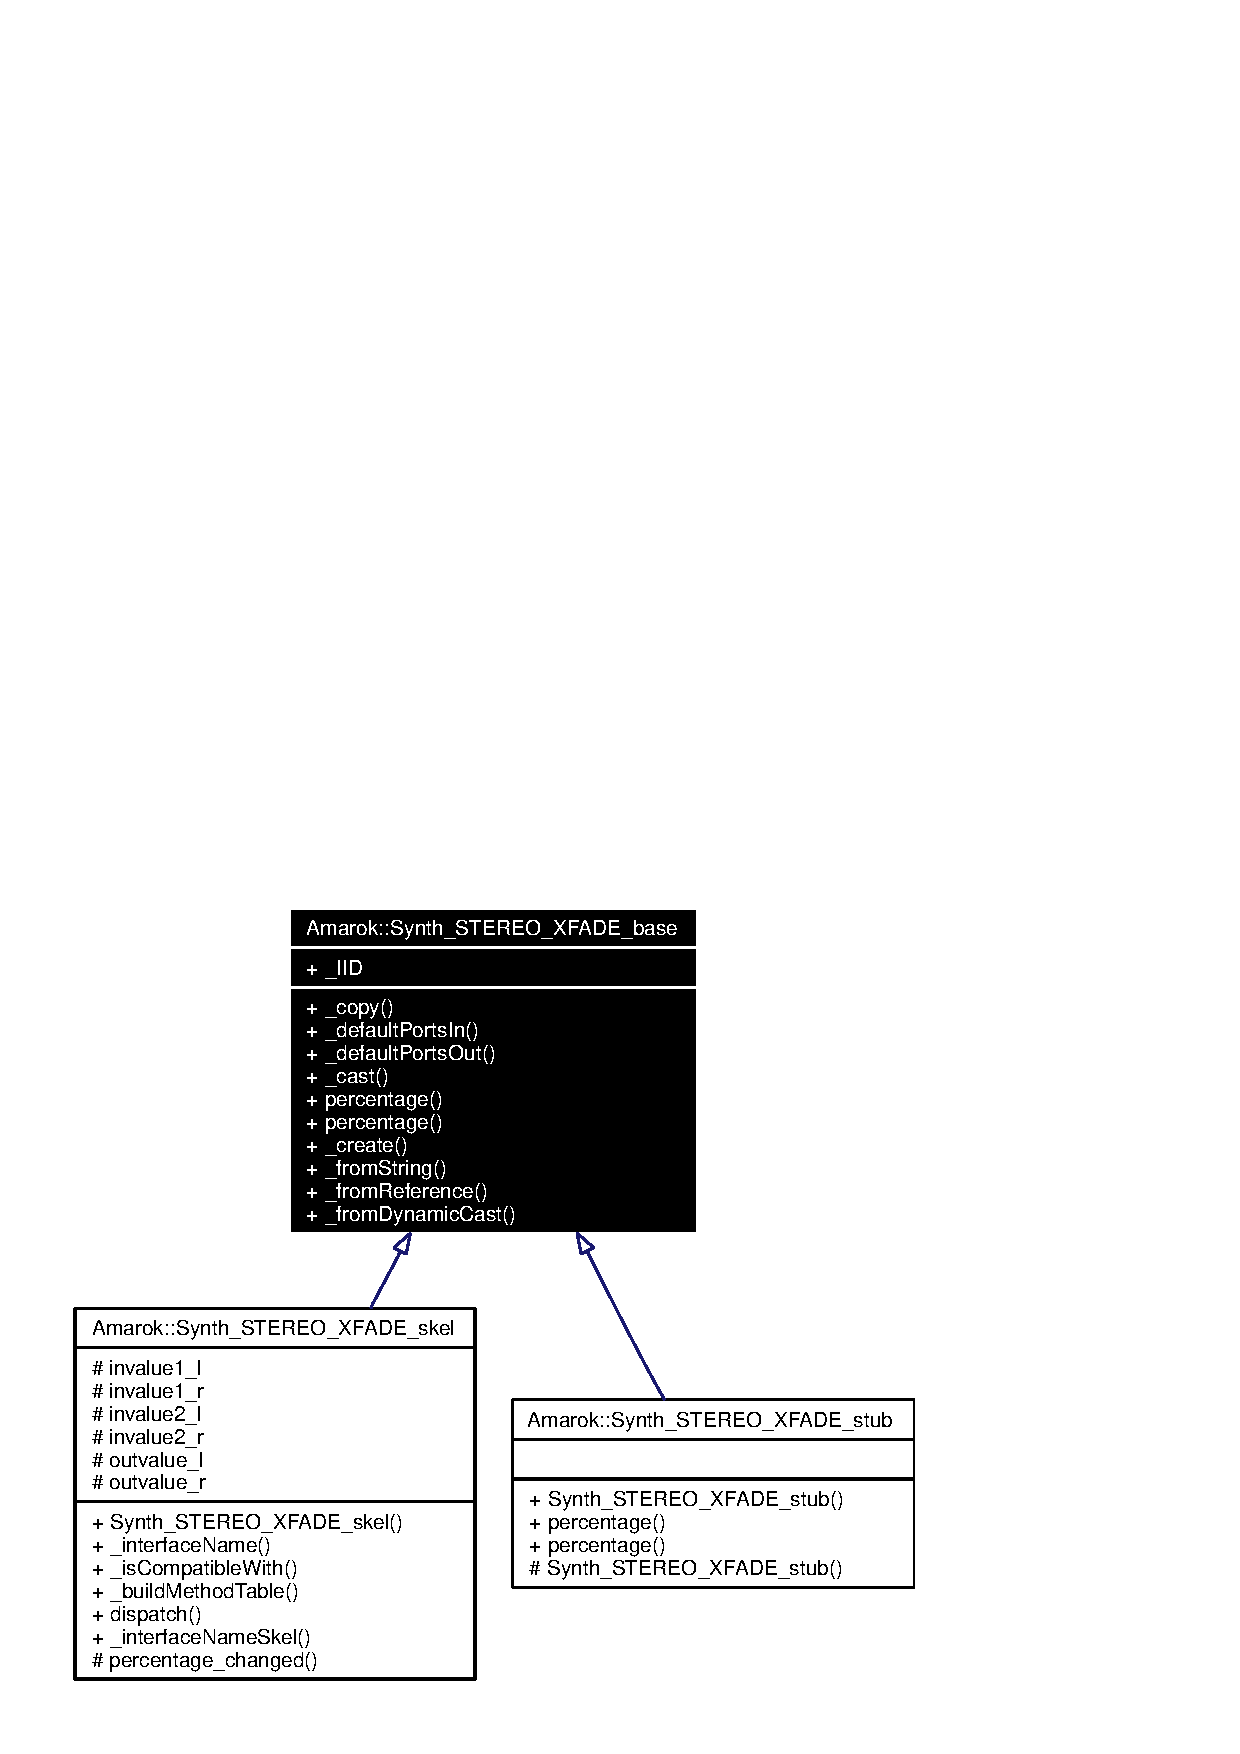
\includegraphics[width=219pt]{classAmarok_1_1Synth__STEREO__XFADE__base__inherit__graph}
\end{center}
\end{figure}
\subsection*{Public Member Functions}
\begin{CompactItemize}
\item 
{\bf Synth\_\-STEREO\_\-XFADE\_\-base} $\ast$ {\bf \_\-copy} ()
\item 
virtual std::vector$<$ std::string $>$ {\bf \_\-default\-Ports\-In} () const 
\item 
virtual std::vector$<$ std::string $>$ {\bf \_\-default\-Ports\-Out} () const 
\item 
void $\ast$ {\bf \_\-cast} (unsigned long iid)
\item 
virtual float {\bf percentage} ()=0
\item 
virtual void {\bf percentage} (float new\-Value)=0
\end{CompactItemize}
\subsection*{Static Public Member Functions}
\begin{CompactItemize}
\item 
{\bf Synth\_\-STEREO\_\-XFADE\_\-base} $\ast$ {\bf \_\-create} (const std::string \&sub\-Class=\char`\"{}Amarok::Synth\_\-STEREO\_\-XFADE\char`\"{})
\item 
{\bf Synth\_\-STEREO\_\-XFADE\_\-base} $\ast$ {\bf \_\-from\-String} (const std::string \&objectref)
\item 
{\bf Synth\_\-STEREO\_\-XFADE\_\-base} $\ast$ {\bf \_\-from\-Reference} (Arts::Object\-Reference ref, bool needcopy)
\item 
{\bf Synth\_\-STEREO\_\-XFADE\_\-base} $\ast$ {\bf \_\-from\-Dynamic\-Cast} (const Arts::Object \&object)
\end{CompactItemize}
\subsection*{Static Public Attributes}
\begin{CompactItemize}
\item 
unsigned long {\bf \_\-IID} = Arts::MCOPUtils::make\-IID(\char`\"{}Amarok::Synth\_\-STEREO\_\-XFADE\char`\"{})
\end{CompactItemize}


\subsection{Member Function Documentation}
\index{Amarok::Synth_STEREO_XFADE_base@{Amarok::Synth\_\-STEREO\_\-XFADE\_\-base}!_cast@{\_\-cast}}
\index{_cast@{\_\-cast}!Amarok::Synth_STEREO_XFADE_base@{Amarok::Synth\_\-STEREO\_\-XFADE\_\-base}}
\subsubsection{\setlength{\rightskip}{0pt plus 5cm}void $\ast$ Amarok::Synth\_\-STEREO\_\-XFADE\_\-base::\_\-cast (unsigned long {\em iid})}\label{classAmarok_1_1Synth__STEREO__XFADE__base_Amarok_1_1Synth__STEREO__XFADE__stuba6}




Definition at line 71 of file amarokarts.cc.

References \_\-IID.

Referenced by \_\-from\-Dynamic\-Cast(), and Amarok::Synth\_\-STEREO\_\-XFADE::\_\-method\_\-call().



\footnotesize\begin{verbatim}72 {
73         if(iid == Amarok::Synth_STEREO_XFADE_base::_IID) return (Amarok::Synth_STEREO_XFADE_base *)this;
74         if(iid == Arts::SynthModule_base::_IID) return (Arts::SynthModule_base *)this;
75         if(iid == Arts::Object_base::_IID) return (Arts::Object_base *)this;
76         return 0;
77 }
\end{verbatim}\normalsize 
\index{Amarok::Synth_STEREO_XFADE_base@{Amarok::Synth\_\-STEREO\_\-XFADE\_\-base}!_copy@{\_\-copy}}
\index{_copy@{\_\-copy}!Amarok::Synth_STEREO_XFADE_base@{Amarok::Synth\_\-STEREO\_\-XFADE\_\-base}}
\subsubsection{\setlength{\rightskip}{0pt plus 5cm}{\bf Synth\_\-STEREO\_\-XFADE\_\-base}$\ast$ Amarok::Synth\_\-STEREO\_\-XFADE\_\-base::\_\-copy ()\hspace{0.3cm}{\tt  [inline]}}\label{classAmarok_1_1Synth__STEREO__XFADE__base_Amarok_1_1Synth__STEREO__XFADE__stuba3}




Definition at line 24 of file amarokarts.h.

Referenced by \_\-from\-Dynamic\-Cast().



\footnotesize\begin{verbatim}24                                                 {
25                 assert(_refCnt > 0);
26                 _refCnt++;
27                 return this;
28         }
\end{verbatim}\normalsize 
\index{Amarok::Synth_STEREO_XFADE_base@{Amarok::Synth\_\-STEREO\_\-XFADE\_\-base}!_create@{\_\-create}}
\index{_create@{\_\-create}!Amarok::Synth_STEREO_XFADE_base@{Amarok::Synth\_\-STEREO\_\-XFADE\_\-base}}
\subsubsection{\setlength{\rightskip}{0pt plus 5cm}{\bf Amarok::Synth\_\-STEREO\_\-XFADE\_\-base} $\ast$ Amarok::Synth\_\-STEREO\_\-XFADE\_\-base::\_\-create (const std::string \& {\em sub\-Class} = \char`\"{}Amarok::Synth\_\-STEREO\_\-XFADE\char`\"{})\hspace{0.3cm}{\tt  [static]}}\label{classAmarok_1_1Synth__STEREO__XFADE__base_Amarok_1_1Synth__STEREO__XFADE__stube0}




Definition at line 8 of file amarokarts.cc.

References \_\-IID.

Referenced by Amarok::Synth\_\-STEREO\_\-XFADE::\_\-Creator().



\footnotesize\begin{verbatim}9 {
10         Arts::Object_skel *skel = Arts::ObjectManager::the()->create(subClass);
11         assert(skel);
12         Amarok::Synth_STEREO_XFADE_base *castedObject = (Amarok::Synth_STEREO_XFADE_base *)skel->_cast(Amarok::Synth_STEREO_XFADE_base::_IID);
13         assert(castedObject);
14         return castedObject;
15 }
\end{verbatim}\normalsize 
\index{Amarok::Synth_STEREO_XFADE_base@{Amarok::Synth\_\-STEREO\_\-XFADE\_\-base}!_defaultPortsIn@{\_\-defaultPortsIn}}
\index{_defaultPortsIn@{\_\-defaultPortsIn}!Amarok::Synth_STEREO_XFADE_base@{Amarok::Synth\_\-STEREO\_\-XFADE\_\-base}}
\subsubsection{\setlength{\rightskip}{0pt plus 5cm}std::vector$<$ std::string $>$ Amarok::Synth\_\-STEREO\_\-XFADE\_\-base::\_\-default\-Ports\-In () const\hspace{0.3cm}{\tt  [virtual]}}\label{classAmarok_1_1Synth__STEREO__XFADE__base_Amarok_1_1Synth__STEREO__XFADE__stuba4}




Definition at line 62 of file amarokarts.cc.



\footnotesize\begin{verbatim}62                                                                           {
63         std::vector<std::string> ret;
64         return ret;
65 }
\end{verbatim}\normalsize 
\index{Amarok::Synth_STEREO_XFADE_base@{Amarok::Synth\_\-STEREO\_\-XFADE\_\-base}!_defaultPortsOut@{\_\-defaultPortsOut}}
\index{_defaultPortsOut@{\_\-defaultPortsOut}!Amarok::Synth_STEREO_XFADE_base@{Amarok::Synth\_\-STEREO\_\-XFADE\_\-base}}
\subsubsection{\setlength{\rightskip}{0pt plus 5cm}std::vector$<$ std::string $>$ Amarok::Synth\_\-STEREO\_\-XFADE\_\-base::\_\-default\-Ports\-Out () const\hspace{0.3cm}{\tt  [virtual]}}\label{classAmarok_1_1Synth__STEREO__XFADE__base_Amarok_1_1Synth__STEREO__XFADE__stuba5}




Definition at line 66 of file amarokarts.cc.



\footnotesize\begin{verbatim}66                                                                            {
67         std::vector<std::string> ret;
68         return ret;
69 }
\end{verbatim}\normalsize 
\index{Amarok::Synth_STEREO_XFADE_base@{Amarok::Synth\_\-STEREO\_\-XFADE\_\-base}!_fromDynamicCast@{\_\-fromDynamicCast}}
\index{_fromDynamicCast@{\_\-fromDynamicCast}!Amarok::Synth_STEREO_XFADE_base@{Amarok::Synth\_\-STEREO\_\-XFADE\_\-base}}
\subsubsection{\setlength{\rightskip}{0pt plus 5cm}{\bf Amarok::Synth\_\-STEREO\_\-XFADE\_\-base} $\ast$ Amarok::Synth\_\-STEREO\_\-XFADE\_\-base::\_\-from\-Dynamic\-Cast (const Arts::Object \& {\em object})\hspace{0.3cm}{\tt  [static]}}\label{classAmarok_1_1Synth__STEREO__XFADE__base_Amarok_1_1Synth__STEREO__XFADE__stube3}




Definition at line 26 of file amarokarts.cc.

References \_\-cast(), \_\-copy(), \_\-from\-String(), and \_\-IID.



\footnotesize\begin{verbatim}27 {
28         if(object.isNull()) return 0;
29 
30         Amarok::Synth_STEREO_XFADE_base *castedObject = (Amarok::Synth_STEREO_XFADE_base *)object._base()->_cast(Amarok::Synth_STEREO_XFADE_base::_IID);
31         if(castedObject) return castedObject->_copy();
32 
33         return _fromString(object._toString());
34 }
\end{verbatim}\normalsize 


Here is the call graph for this function:\begin{figure}[H]
\begin{center}
\leavevmode
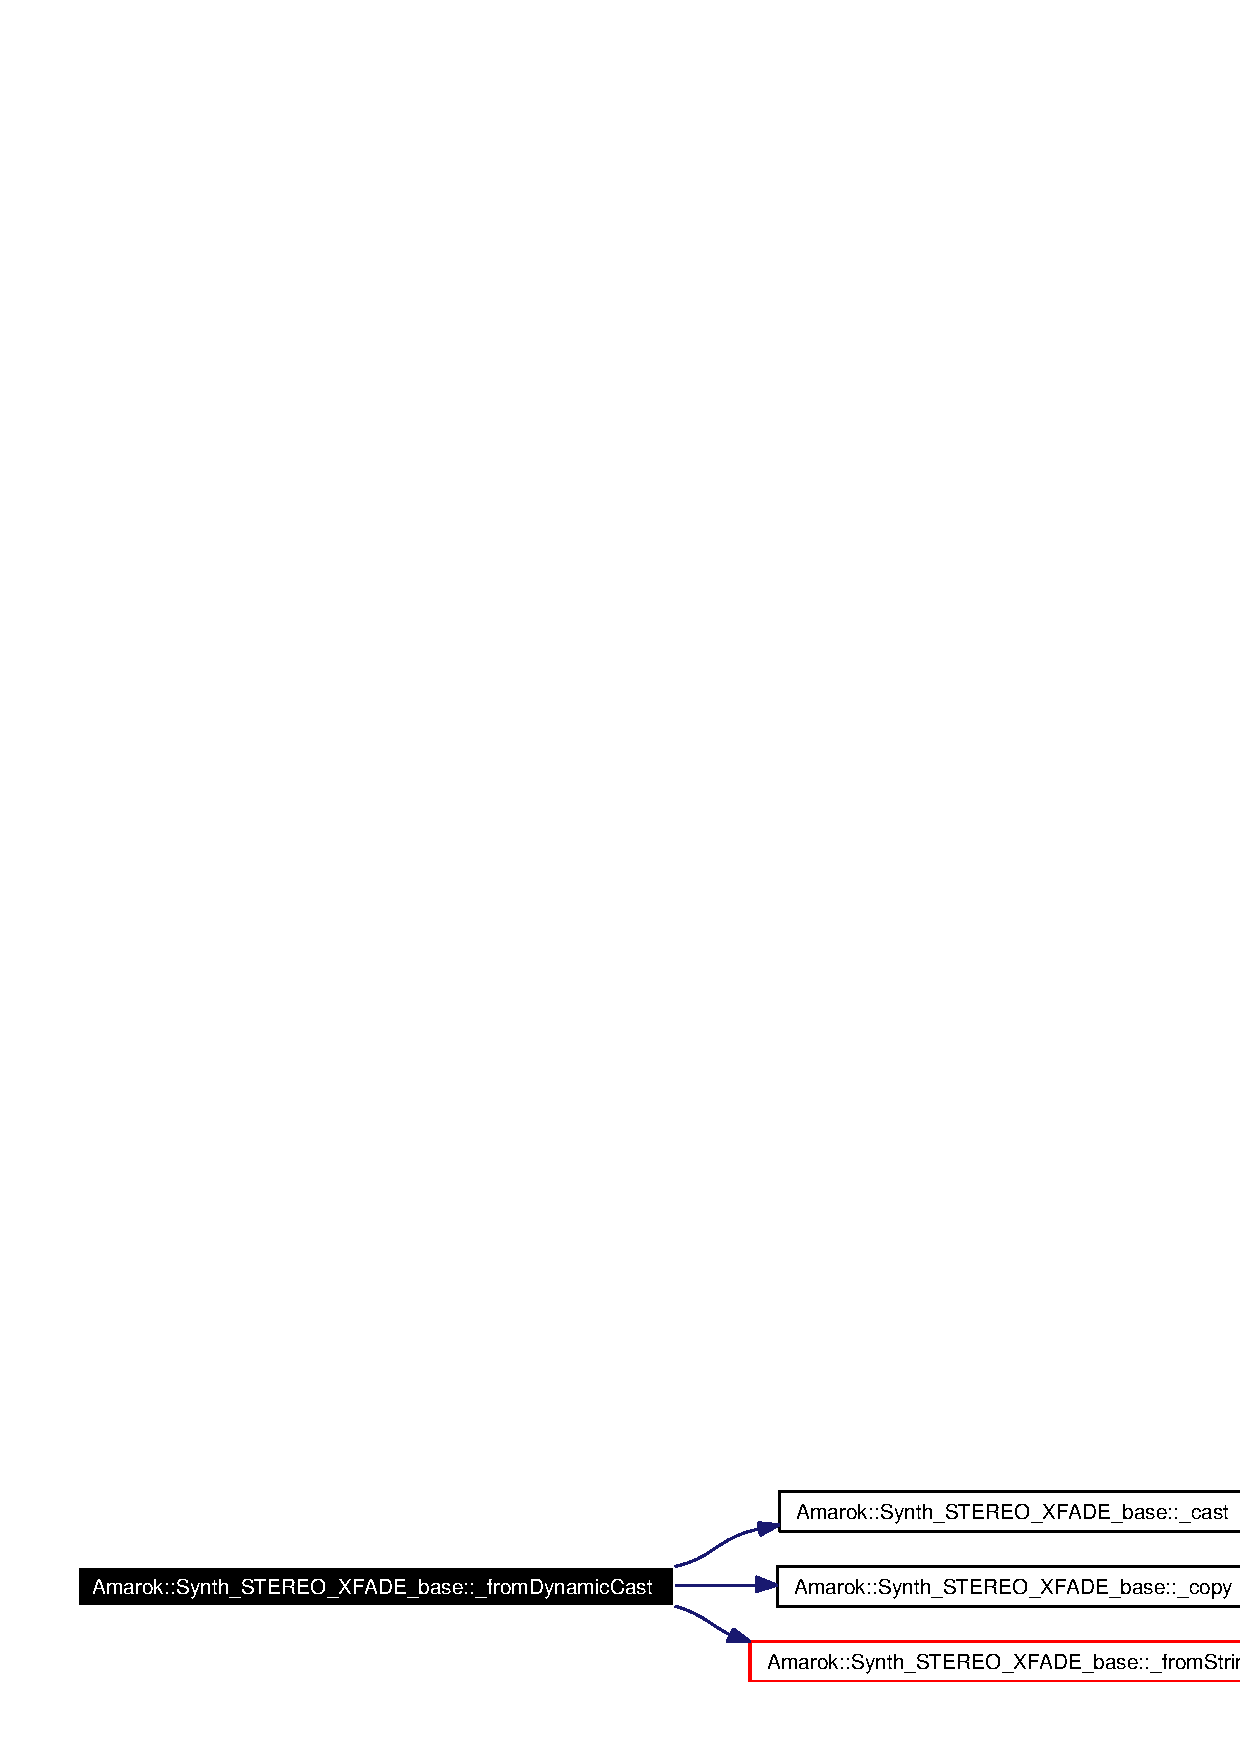
\includegraphics[width=307pt]{classAmarok_1_1Synth__STEREO__XFADE__base_Amarok_1_1Synth__STEREO__XFADE__stube3_cgraph}
\end{center}
\end{figure}
\index{Amarok::Synth_STEREO_XFADE_base@{Amarok::Synth\_\-STEREO\_\-XFADE\_\-base}!_fromReference@{\_\-fromReference}}
\index{_fromReference@{\_\-fromReference}!Amarok::Synth_STEREO_XFADE_base@{Amarok::Synth\_\-STEREO\_\-XFADE\_\-base}}
\subsubsection{\setlength{\rightskip}{0pt plus 5cm}{\bf Amarok::Synth\_\-STEREO\_\-XFADE\_\-base} $\ast$ Amarok::Synth\_\-STEREO\_\-XFADE\_\-base::\_\-from\-Reference (Arts::Object\-Reference {\em ref}, bool {\em needcopy})\hspace{0.3cm}{\tt  [static]}}\label{classAmarok_1_1Synth__STEREO__XFADE__base_Amarok_1_1Synth__STEREO__XFADE__stube2}




Definition at line 36 of file amarokarts.cc.

Referenced by \_\-from\-String().



\footnotesize\begin{verbatim}37 {
38         Amarok::Synth_STEREO_XFADE_base *result;
39         result = (Amarok::Synth_STEREO_XFADE_base *)Arts::Dispatcher::the()->connectObjectLocal(r,"Amarok::Synth_STEREO_XFADE");
40         if(result)
41         {
42                 if(!needcopy)
43                         result->_cancelCopyRemote();
44         }
45         else
46         {
47                 Arts::Connection *conn = Arts::Dispatcher::the()->connectObjectRemote(r);
48                 if(conn)
49                 {
50                         result = new Amarok::Synth_STEREO_XFADE_stub(conn,r.objectID);
51                         if(needcopy) result->_copyRemote();
52                         result->_useRemote();
53                         if (!result->_isCompatibleWith("Amarok::Synth_STEREO_XFADE")) {
54                                 result->_release();
55                                 return 0;
56                         }
57                 }
58         }
59         return result;
60 }
\end{verbatim}\normalsize 
\index{Amarok::Synth_STEREO_XFADE_base@{Amarok::Synth\_\-STEREO\_\-XFADE\_\-base}!_fromString@{\_\-fromString}}
\index{_fromString@{\_\-fromString}!Amarok::Synth_STEREO_XFADE_base@{Amarok::Synth\_\-STEREO\_\-XFADE\_\-base}}
\subsubsection{\setlength{\rightskip}{0pt plus 5cm}{\bf Amarok::Synth\_\-STEREO\_\-XFADE\_\-base} $\ast$ Amarok::Synth\_\-STEREO\_\-XFADE\_\-base::\_\-from\-String (const std::string \& {\em objectref})\hspace{0.3cm}{\tt  [static]}}\label{classAmarok_1_1Synth__STEREO__XFADE__base_Amarok_1_1Synth__STEREO__XFADE__stube1}




Definition at line 17 of file amarokarts.cc.

References \_\-from\-Reference().

Referenced by \_\-from\-Dynamic\-Cast().



\footnotesize\begin{verbatim}18 {
19         Arts::ObjectReference r;
20 
21         if(Arts::Dispatcher::the()->stringToObjectReference(r,objectref))
22                 return Amarok::Synth_STEREO_XFADE_base::_fromReference(r,true);
23         return 0;
24 }
\end{verbatim}\normalsize 


Here is the call graph for this function:\begin{figure}[H]
\begin{center}
\leavevmode
\includegraphics[width=300pt]{classAmarok_1_1Synth__STEREO__XFADE__base_Amarok_1_1Synth__STEREO__XFADE__stube1_cgraph}
\end{center}
\end{figure}
\index{Amarok::Synth_STEREO_XFADE_base@{Amarok::Synth\_\-STEREO\_\-XFADE\_\-base}!percentage@{percentage}}
\index{percentage@{percentage}!Amarok::Synth_STEREO_XFADE_base@{Amarok::Synth\_\-STEREO\_\-XFADE\_\-base}}
\subsubsection{\setlength{\rightskip}{0pt plus 5cm}virtual void Amarok::Synth\_\-STEREO\_\-XFADE\_\-base::percentage (float {\em new\-Value})\hspace{0.3cm}{\tt  [pure virtual]}}\label{classAmarok_1_1Synth__STEREO__XFADE__base_Amarok_1_1Synth__STEREO__XFADE__skela10}




Implemented in {\bf Amarok::Synth\_\-STEREO\_\-XFADE\_\-stub} {\rm (p.\,\pageref{classAmarok_1_1Synth__STEREO__XFADE__stub_Amarok_1_1Synth__STEREO__XFADE__stuba2})}.\index{Amarok::Synth_STEREO_XFADE_base@{Amarok::Synth\_\-STEREO\_\-XFADE\_\-base}!percentage@{percentage}}
\index{percentage@{percentage}!Amarok::Synth_STEREO_XFADE_base@{Amarok::Synth\_\-STEREO\_\-XFADE\_\-base}}
\subsubsection{\setlength{\rightskip}{0pt plus 5cm}virtual float Amarok::Synth\_\-STEREO\_\-XFADE\_\-base::percentage ()\hspace{0.3cm}{\tt  [pure virtual]}}\label{classAmarok_1_1Synth__STEREO__XFADE__base_Amarok_1_1Synth__STEREO__XFADE__skela9}




Implemented in {\bf Amarok::Synth\_\-STEREO\_\-XFADE\_\-stub} {\rm (p.\,\pageref{classAmarok_1_1Synth__STEREO__XFADE__stub_Amarok_1_1Synth__STEREO__XFADE__stuba1})}.

Referenced by Amarok::Synth\_\-STEREO\_\-XFADE::percentage().

\subsection{Member Data Documentation}
\index{Amarok::Synth_STEREO_XFADE_base@{Amarok::Synth\_\-STEREO\_\-XFADE\_\-base}!_IID@{\_\-IID}}
\index{_IID@{\_\-IID}!Amarok::Synth_STEREO_XFADE_base@{Amarok::Synth\_\-STEREO\_\-XFADE\_\-base}}
\subsubsection{\setlength{\rightskip}{0pt plus 5cm}unsigned long {\bf Amarok::Synth\_\-STEREO\_\-XFADE\_\-base::\_\-IID} = Arts::MCOPUtils::make\-IID(\char`\"{}Amarok::Synth\_\-STEREO\_\-XFADE\char`\"{})\hspace{0.3cm}{\tt  [static]}}\label{classAmarok_1_1Synth__STEREO__XFADE__base_Amarok_1_1Synth__STEREO__XFADE__stubs0}




Definition at line 180 of file amarokarts.cc.

Referenced by \_\-cast(), \_\-create(), and \_\-from\-Dynamic\-Cast().

The documentation for this class was generated from the following files:\begin{CompactItemize}
\item 
{\bf amarokarts.h}\item 
{\bf amarokarts.cc}\end{CompactItemize}
